\documentclass[tikz]{standalone}
\usetikzlibrary{arrows, positioning}
\tikzset{
  treenode/.style = {align=center, inner sep=1pt, text centered,
    font=\sffamily},
  arn_b/.style = {treenode, circle, white, font=\sffamily\bfseries, draw=black,
    fill=black, text width=1.5em},% arbre rouge noir, noeud noir
  arn_r/.style = {treenode, circle, red, draw=red, 
    text width=1.5em, very thick}% arbre rouge noir, noeud rouge
}

\begin{document}

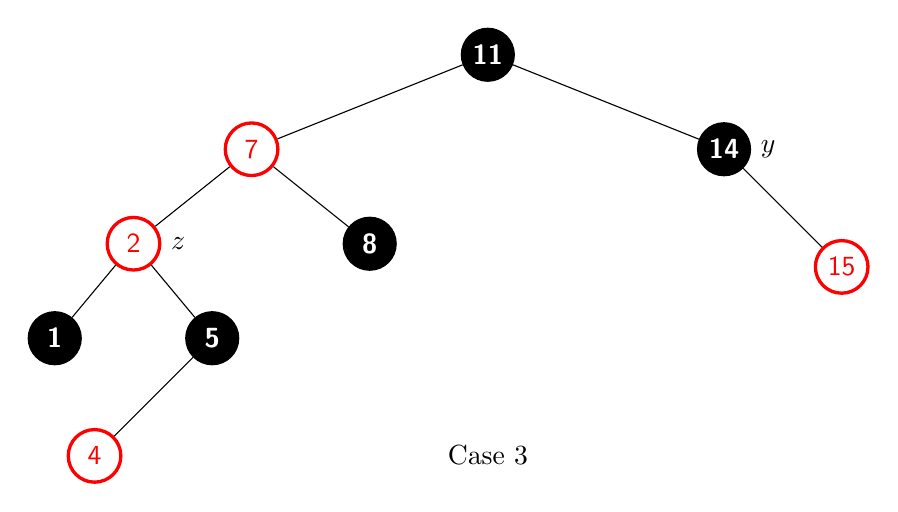
\begin{tikzpicture}[level/.style={sibling distance = 6cm/#1,
    level distance = 1.2cm}] 
  \node (root) [arn_b] {11}
      child{ node [arn_r] {7} 
              child{ node (cn2) [arn_r] {2} 
                child{ node [arn_b] {1}}
                child{ node (cn5) [arn_b] {5} 
                    child{ node [arn_r, below left=of cn5] {4} }
                }
              }
              child{ node [arn_b] {8}}
            }                            
      child{ node (cn14) [arn_b] {14}
          child{ node [arn_r, below right=of cn14] {15}}
      }
      ;
  \node [right] at (cn2.east) {$z$};
  \node [right] at (cn14.east) {$y$};
  \node [below=of root, yshift=-3.5cm] {Case 3};
\end{tikzpicture}

\end{document}